% ----- formatovani dokumentu -----------------------------------------------
\documentclass[12pt,a4paper,titlepage,final]{report}
\usepackage[utf8]{inputenc}
\usepackage[T1, IL2]{fontenc}
\usepackage{graphicx}
\usepackage{epstopdf}
\usepackage[margin=2cm]{caption}
\usepackage[top=3cm, left=2cm, right=2cm, text={17cm, 24cm}, ignorefoot]{geometry}
\usepackage[usenames,dvipsnames]{color}
\usepackage{url}
\usepackage{setspace}
\usepackage{amsmath}
\singlespacing
\usepackage[square, numbers]{natbib} 
\pagestyle{plain}
\pagenumbering{arabic}
\setcounter{page}{1}
\setcounter{secnumdepth}{-1}
\setlength{\parindent}{1cm}	
\usepackage{natbib}


% ----- vyberte jazyk -------------------------------------------------------
\usepackage[english,czech]{babel}
%\usepackage[english]{babel}

% ----- dopiste titulky -----------------------------------------------------
\newcommand\Course{Hardware/Software Codesign}
\newcommand\WorkTitle{Vestavěný systém pro filtraci a segmentaci obrazu}
\newcommand\AuthorA{Pavel Macenauer}
\newcommand\AuthorAEmail{xmacen02}
\newcommand\Faculty{Fakulta Informačních Technologií}
\newcommand\School{Vysoké Učení Technické v Brně}

\usepackage[
pdftitle={\WorkTitle},
pdfauthor={\AuthorA},
bookmarks=true,
colorlinks=true,
breaklinks=true,
urlcolor=blue,
citecolor=blue,
linkcolor=blue,
unicode=true,
]
{hyperref}


% ----- titulni strana ------------------------------------------------------

\begin{document}
	\begin{titlepage}
	\begin{center}
		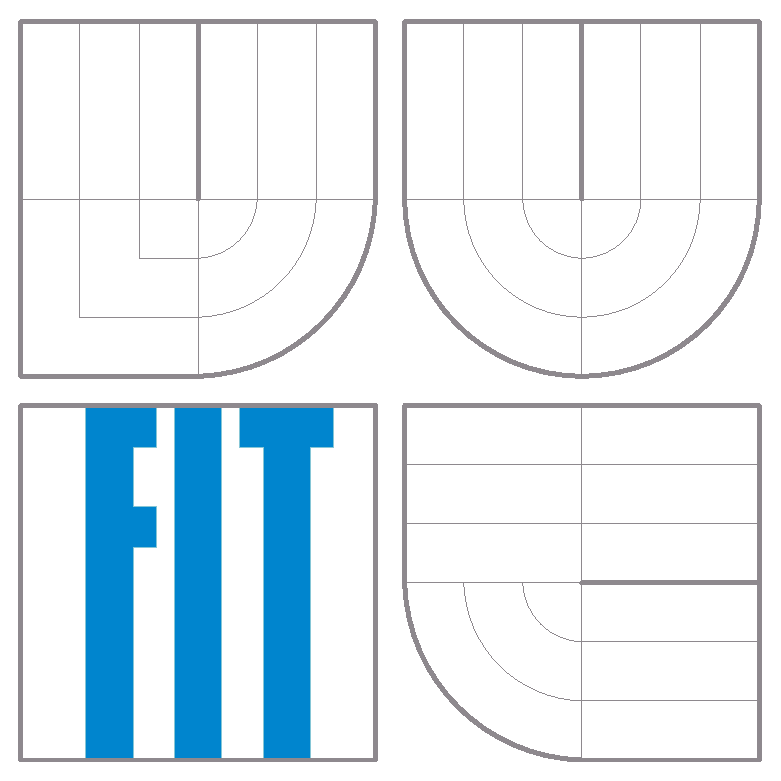
\includegraphics[height=5cm]{images/logo.eps}
	\end{center}
	\vfill
	\begin{center}
		\begin{Large}
			\Course\\
		\end{Large}
		\bigskip
		\begin{Huge}
			\WorkTitle\\
		\end{Huge}
	\end{center}
	\vfill
	\begin{center}
		\begin{large}
			\today
		\end{large}
	\end{center}
	\vfill
	\begin{flushleft}
		\begin{large}
			\begin{tabular}{lll}
				Autoři: & \AuthorA, & \url{\AuthorAEmail} \\
				        &  \\
				& & \\
				& \Faculty \\
				& \School \\
			\end{tabular}
		\end{large}
	\end{flushleft}
\end{titlepage}		
	
% ----- obsah --------------------------------------------------------------
	
\tableofcontents

% ----- zadani -------------------------------------------------------------
\newpage
\section{Analýza algoritmu z programu gprof}

\begin{table}[h!]
	\begin{center}
    \begin{tabular}{ | p{3cm} | p{6cm} |}
    \hline
    Čas [\%] & Jméno funkce
    \\ \hline
    
    58,97 & \verb|median|
    \\ \hline
	11,5 & \verb|gen_pixel|
	\\ \hline
	8,67 & \verb|clip_window|
	\\ \hline
	5,77 & \verb|shift_window|
	\\ \hline
	4,94 & \verb|buffer|
	\\ \hline
	4,45 & \verb|pixel_processing|
	\\ \hline
	2,69 & \verb|system_input|
	\\ \hline
	1,6 & \verb|main|
	\\ \hline
	0,67 & \verb|thresholding|
	\\ \hline
	0,32 & \verb|histogram_clean|
	\\ \hline
	0,23 & \verb|otsu|
	\\ \hline
	0,19 & \verb|update_base_pos|
	\\ \hline
    	
	
    \end{tabular}
	\end{center}	
	\caption{Podíl celkového času běhu programu pro jednotlivé funkce}  
\end{table}

\begin{center}
	\captionsetup{type=figure}
		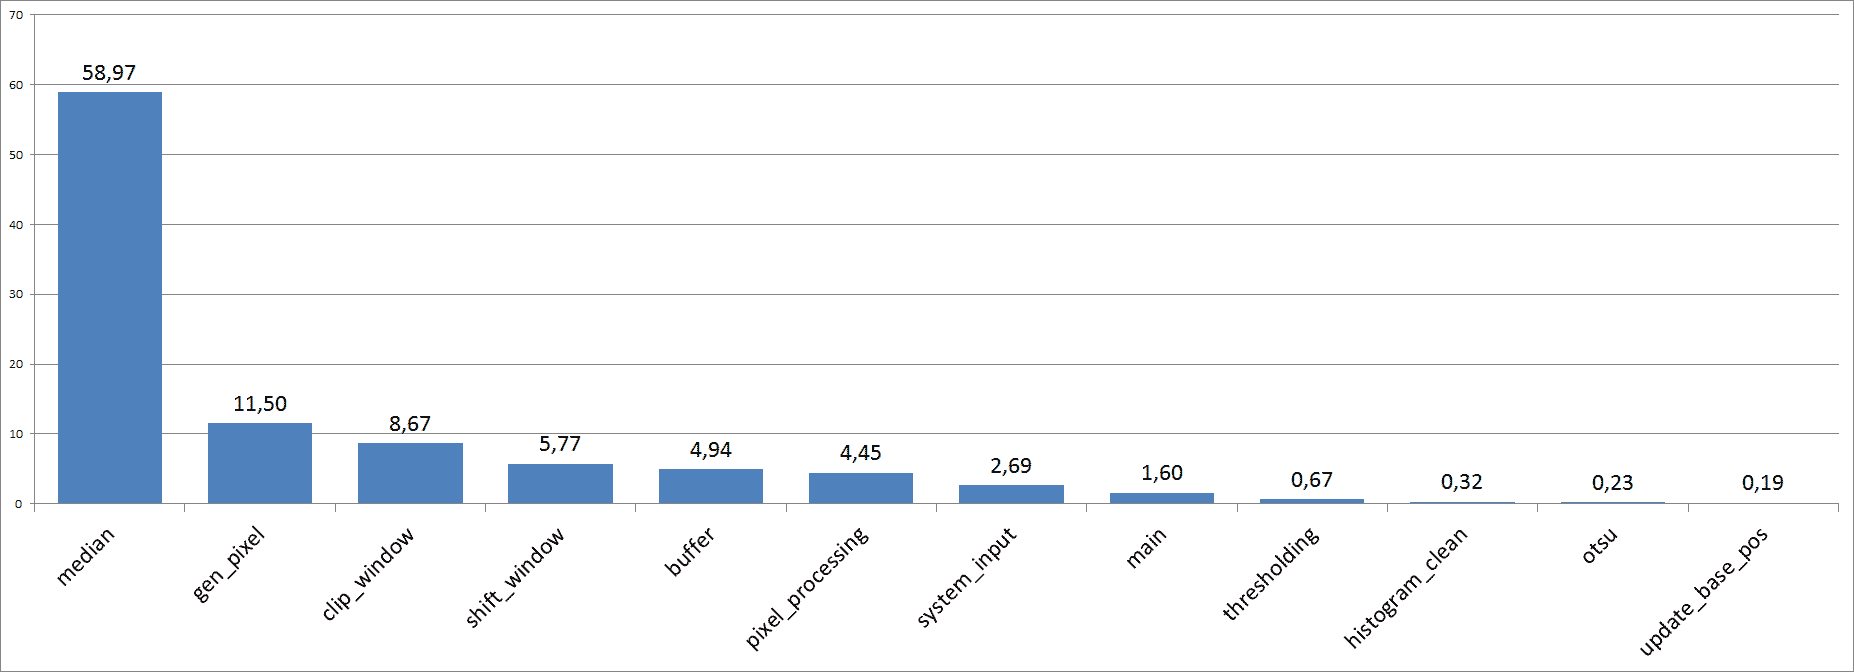
\includegraphics[width=16cm]{images/graf.png}
	\captionof{figure}{Podíl celkového času běhu programu pro jednotlivé funkce}
\end{center}

\newpage
%---------------------------------------------------------------------------
\section{Rozdělení aplikace mezi software a hardware}

\begin{table}[h!]
	\begin{center}
    \begin{tabular}{ | p{3cm} | p{6cm} |}
    \hline
    Původní funkce na MCU & Přesunuto na HW
    \\ \hline
    
   	otsu & \textcolor{red}{\textbf{NE}}	
	\\ \hline
	median & \textcolor{ForestGreen}{ANO}
	\\ \hline
	buffer & \textcolor{ForestGreen}{ANO}
	\\ \hline
	clip\_window & \textcolor{ForestGreen}{ANO}
	\\ \hline
	shift\_window & \textcolor{ForestGreen}{ANO}
	\\ \hline
	system\_input & \textcolor{ForestGreen}{ANO}
	\\ \hline
	histogram\_clean & \textcolor{red}{\textbf{NE}}
	\\ \hline
	thresholding & \textcolor{ForestGreen}{ANO}
	\\ \hline
	print\_results & \textcolor{red}{\textbf{NE}}
	\\ \hline
	pixel\_processing & \textcolor{ForestGreen}{ANO}
	\\ \hline
	update\_base\_pos & \textcolor{ForestGreen}{ANO, realizováno komponentou Generátor pixelů}
	\\ \hline
	gen\_pixel & \textcolor{ForestGreen}{ANO, realizováno komponentou Generátor pixelů}
	\\ \hline
    	
	
    \end{tabular}
	\end{center}	
	\caption{Rozdělení aplikace mezi software a hardware}  
\end{table}
	


%---------------------------------------------------------------------------
\section{Využití adresového prostoru sdílené paměti}

\begin{table}[h!]
	\begin{center}
    \begin{tabular}{ | p{1.5cm} | p{4cm} | p{5cm} | p{1.5cm} |}
    \hline
    Adresa & Jméno & Poznámka & MCU
    \\ \hline
    
   	0 & \verb|MCU_DATA_HIST0| & První položka histogramu
   		& \textcolor{ForestGreen}{vstup}
	\\ \hline
	1 & \verb|MCU_DATA_HIST1| &
		& \textcolor{ForestGreen}{vstup}
	\\ \hline
	2 & \verb|MCU_DATA_HIST2| &
		& \textcolor{ForestGreen}{vstup}
	\\ \hline
	3 & \verb|MCU_DATA_HIST3| &
		& \textcolor{ForestGreen}{vstup}
	\\ \hline
	4 & \verb|MCU_DATA_HIST4| &
		& \textcolor{ForestGreen}{vstup}
	\\ \hline
	5 & \verb|MCU_DATA_HIST5| &
		& \textcolor{ForestGreen}{vstup}
	\\ \hline
	6 & \verb|MCU_DATA_HIST6| &
		& \textcolor{ForestGreen}{vstup}
	\\ \hline
	7 & \verb|MCU_DATA_HIST7| & Poslední položka histogramu
	& \textcolor{ForestGreen}{vstup}
	\\ \hline
	8 & \verb|MCU_DATA_THRESHOLD| & MCU zde ukládá nově vypočtený práh, FPGA si ho načítá
	& \textcolor{red}{výstup}
	\\ \hline
	9 & \verb|MCU_FLAG_OTSU_START| & Příznak, který určuje, že se má vypočíst nová hodnota prahu & \textcolor{ForestGreen}{vstup}
	\\ \hline    	
	
    \end{tabular}
	\end{center}	
	\caption{Využití adresového prostoru sdílené paměti}  
\end{table}


%---------------------------------------------------------------------------
\section{Vlastnosti obvodu uvnitř FPGA}

\begin{itemize}
	\item Inicializační interval smyčky \verb|(PIPELINE_INIT_INTERVAL)| 4
	\item Latence obvodu 4 (při periodě 40 $ns$)
\end{itemize}

\begin{table}[h!]
	\begin{center}
    \begin{tabular}{ | p{4cm} | p{4cm} | p{4cm} |}    
	\hline    
   	Number of Slice Flip Flops & 394 out of 1,536 & 25\% 
	\\ \hline
	Number of 4 input LUTs & 914 out of 1,536 & 59\%	
	\\ \hline
	Number of occupied Slices & 610 out of 768 & 79\% 
	\\ \hline
	Total Number of 4 input LUTs & 1,002 out of 1,536 & 65\%	
	\\ \hline 
	Number used as logic & 914 &
	\\ \hline 
    Number used as a route-thru & 88 &
	\\ \hline     	
	
    \end{tabular}
	\end{center}	
	\caption{Využití a rozdělení obvodu}  
\end{table}



%---------------------------------------------------------------------------
\section{Porovnání softwarové a rozdělené implementace}


\begin{table}[h!]
	\begin{center}
    \begin{tabular}{ | p{4cm} | p{4cm} | p{4cm} |}    
	\hline 
	& Software & Rozdělená aplikace   
	\\ \hline
	Doba zpracování pixelu [$\mu s$] & 182 & 0,16
	\\ \hline 
	Zpracovaných pixelů za sekundu [px/s] & 5494 & 6250000
	\\ \hline 
	Zrychlení & 1x & 1137x
	\\ \hline     
	
    \end{tabular}
	\end{center}	
	\caption{Porovnání čistě softwarové a rozdělené aplikace mezi hardware a software}  
\end{table}

\section{Shrnutí}

Ukázalo se, že čistě softwarová implementace je v praxi nepoužitelná, protože řešení vygeneruje 0,07 framů za sekundu (fps) při rozlišení 320x240. Při použití FPGA (hardwaru) se aplikace výrazně zrychlila a byla schopná vygenerovat 81 fps, což splňuje požadavek minimálně 60 fps.

Pravděpodobně by šlo přesunout i výpočet prahu metodou otsu z MCU na FPGA, ale výsledek by to mělo pouze na výslednou kvalitu obrazu, protože bychom byli schopni aktualizovat práh častěji. Není to tak potřeba a může probíhat víceméně asynchronně na MCU.

Úzkým hrdlem mi přišlo především omezení počtu zápisu a čtení do/ze sdílené paměti, kdy se musely redukovat veškeré pomocné příznaky na minimum. Pro složitější algoritmy zpracování obrazu, využívající více zdrojů, by se tak musel výrazně zvýšit inicializační interval smyčky.

\end{document}

